\begin{frame}[t]
    \frametitle{The Minimal Bounding Volume Hierarchy}
    \begin{block}{The Minimal Bounding Volume Hierarchy (MVH)}
        Минимальная иерархия ограничевающих объемов - полное k-арное дерево BVH, которое хранится в массиве
        и индексируется как heap.
        Каждый узел либо листовой, либо имеет k дочерних.
    \end{block}
    Принципы, используемые для этого компактного представления BVH:
    \begin{itemize}
        \item
            Удаление дочерних и примитивных указателей \textbf{неявным индексированием}
        \item
            \textbf{Сокращение информации}, которая хранится для каждого BV
    \end{itemize}

\end{frame}

\begin{frame}[t]
    \frametitle{Неявное индексировние}
    \framesubtitle{Minimal Bounding Volume Hierarchy}

    \begin{columns}
        \column{0.5\textwidth}
        \begin{block}{}
            Индексы дочерних узлов $i$-ого узла между $i*k+1$ и $i*k + k$
        \end{block}

        В статье-источнике $k=2$, то есть дерево - бинарное.

        Обозначим кол-во примитивов на узел $n$. И пусть листовые узлы начинаются с индекса $l$.

        \begin{block}{}
            $primID = (i - l) * n$ - будет индекс первого примитива в массиве примитивов для $i$-го узла (если он листовой, то $i > l$).
        \end{block}
        \column{0.5\textwidth}
        \begin{figure}
            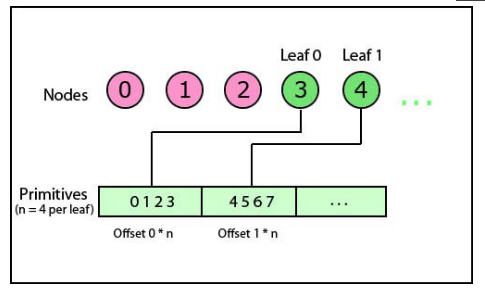
\includegraphics[keepaspectratio, width=\textwidth]{res/mem_layout_mvh.png}
        \end{figure}
        \begin{figure}
            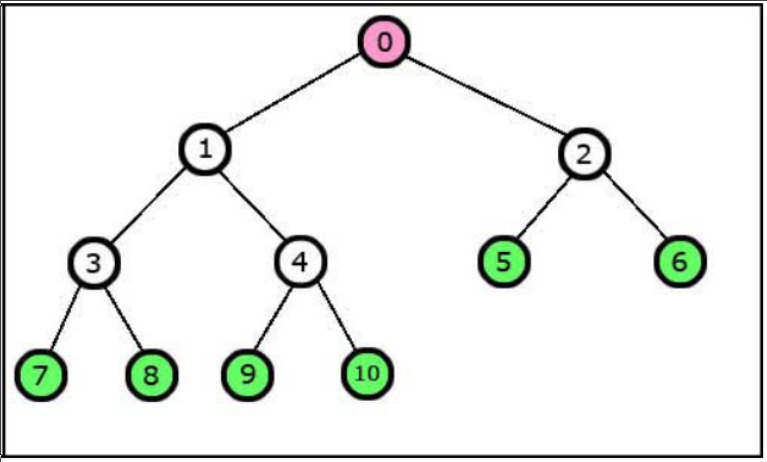
\includegraphics[keepaspectratio, width=0.9\textwidth]{res/tree_mvh.png}
        \end{figure}
    \end{columns}

\end{frame}

\begin{frame}[t]
    \frametitle{Сокращение хранимых данных для узла MVH}
    \framesubtitle{Minimal Bounding Volume Hierarchy}
    \begin{columns}
        \column{0.7\textwidth}
        Выделим для узла всего 2 бита. Получим 4 возможных варианта для получившегося дочернего узла:
        \begin{itemize}
            \item
                No-Cut: if no surface reduction is possible for this node
            \item
                Left-Cut: if the minimum slab is increased
            \item
                Right-Cut: if the maximum slab is decreased
            \item
                Both-Cut: if the Left-Cut and Right-Cut is used
        \end{itemize}
        \column{0.3\textwidth}
        \begin{figure}
            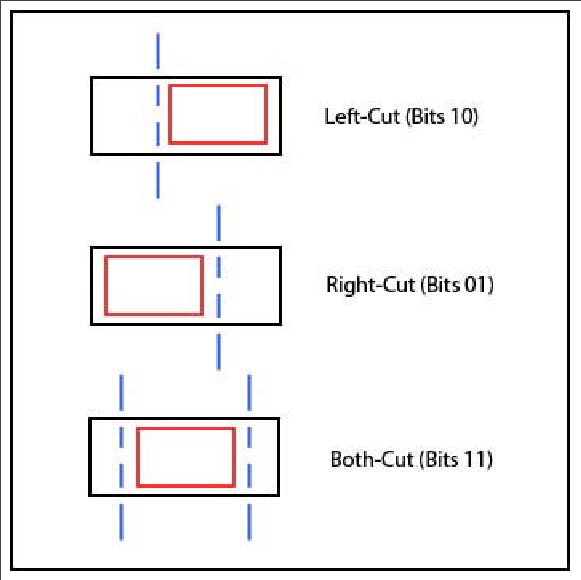
\includegraphics[keepaspectratio, width=\textwidth]{res/splitting_mvh.png}
        \end{figure}
    \end{columns}
    \begin{block}{}
        Каждый раз мы используем фиксированный reduction factor $\zeta$
        Лучшие результаты с $\zeta \in [ 0.30, 0.35]$
    \end{block}

\end{frame}

\begin{frame}
    \frametitle{Построение MVH. Алгоритм}
    \framesubtitle{Minimal Bounding Volume Hierarchy}
    \begin{enumerate}
        \setcounter{enumi}{-1}
        \item
            Input: P - кол-во примитивов в сцене, обычное AABB BVH
        \item
            Дублируем последний примитив пока $P$ не станет $ P \% n = 0$
        \item
            Сколько узлов всего? Для $k = 2$ кол-во узлов $2(P/n) -1$
        \item
            Сколько узлов в каждом поддереве?
            \begin{itemize}
                \item[$-$]
                    Присваиваем всем листьям их кол-во примитивов
                \item[$-$]
                    Суммируем bottom-up, пока не дойдем до корня
            \end{itemize}
        \item
            Пусть всего $N$ узлов. Тогда аллоцируем массив длины $2N$ из \textit{int32}
        \item
            MVH строится с использованием object median split, где
            \textbf{процесс разделения} использует предварительно вычисленные количества примитивов для
            разделения списка объектов на две части
    \end{enumerate}
\end{frame}

\begin{frame}
    \frametitle{Процесс разделения BV}
    \framesubtitle{Minimal Bounding Volume Hierarchy}
    \begin{enumerate}
        \item
            Отсекаем от рамки родителя способами 01, 10, 11 и сравниваем с реальным BV для текущего списка примитивов
        \item
            Если один из способов нам подходит - записываем в массив эти 2 бита.
        \item
            Как только дошли до листа - заносим примитивы в массив примитивов под соответствующими индексами
    \end{enumerate}
    \begin{block}{}
        На каждом этапе разделения выбирается ось, вдоль которой располагаются самые длинные грани приближенного AABB
    \end{block}
    \begin{block}{Глобальные параметры}
        \begin{itemize}
            \item
                Root's BB
            \item
                Reduction factor $\zeta$
        \end{itemize}
    \end{block}
\end{frame}

\begin{frame}[t]{Пример построения MVH}
    \framesubtitle{Minimal Bounding Volume Hierarchy}
    \begin{figure}
        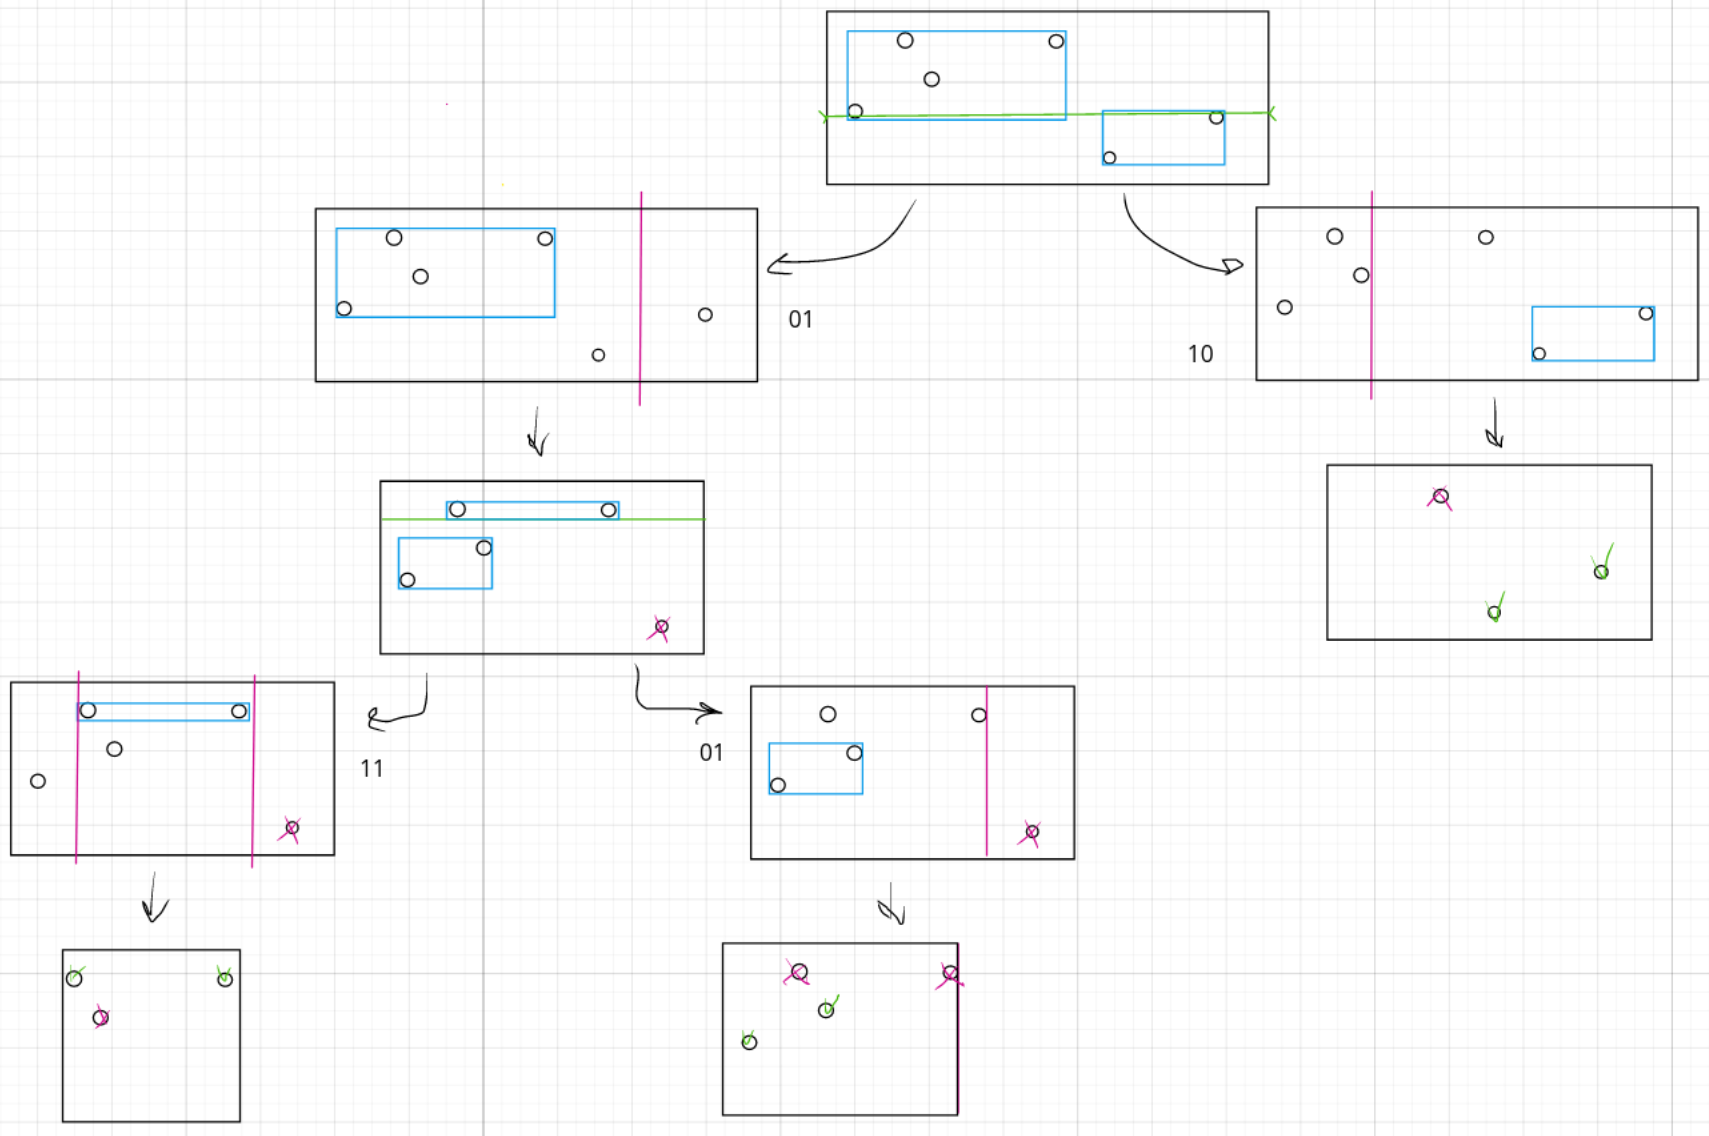
\includegraphics[keepaspectratio, width=\textwidth]{res/mvh.png}
    \end{figure}
\end{frame}

\begin{frame}[fragile]
    \frametitle{Обход MVH}
    \framesubtitle{Minimal Bounding Volume Hierarchy}

    Алгоритм обхода такой же, как и для Single Slab, однако строить splitting plane приходится на самом этапе обхода.

    \begin{lstlisting}[language=C++,basicstyle=\ttfamily,keywordstyle=\color{blue}]
float minTab[4] = { 0.0f, zeta, 0.0f, zeta };
float maxTab[4] = { 0.0f, 0.0f, zeta, zeta };
bool intersect(Ray& r, float& tHit, int* mvhArray,
        int node, AABB& parent,
        float tNear, float tFar) {
    // reconstruct AABB
    vec3 size = parent.max - parent.min;
    char axis = GetAxisOfMaximumExtent(size);
    char bitID = GetNodeCut(node);
    parent.min[axis] += size[axis]*minTab[bitID];
    parent.max[axis] -= size[axis]*maxTab[bitID];

    ...
    \end{lstlisting}

\end{frame}

\begin{frame}[fragile]
    \frametitle{Обход MVH (продолжение)}
    \framesubtitle{Minimal Bounding Volume Hierarchy}

    \begin{lstlisting}[language=C++,basicstyle=\ttfamily,keywordstyle=\color{blue}]
    ...
    // intersection
    float tmin, tmax;
    parent.intersect(r, tmin, tmax, axis);
    float tNear = max(min(tmin, tmax), tNear);
    float tFar = min(max(tmin, tmax), tFar);
    return ((tNear <= tFar) && (tNear <= tHit));
}

char GetNodeCut(int node, int* mvhArray) {
    int iIndex = node >> 4;
    int iShift = (node & 15) << 1;
    return ((mvhArray[iIndex] >> iShift) & 0x3);
}
    \end{lstlisting}

\end{frame}

\begin{frame}[t]
    \frametitle{Двухуровневая MVH. TLAS и BLAS}
    \framesubtitle{Minimal Bounding Volume Hierarchy}
    \begin{block}{Идея}
        \begin{itemize}
            \item
                Половина всех затрат памяти приходится на последний уровень дерева BVH (вдвое больше узлов)
            \item
                Большинство лучей пересакают верхние уровни дерева - надо сделать их качественными
        \end{itemize}
    \end{block}
    \begin{block}{Top level acceleration structure (TLAS)}
        Верхний уровень в несжатом BVH формате, оптимизированный с помощью затратного по времени SAH
    \end{block}
    \begin{block}{Bottom level acceleration structure (BLAS)}
        Нижний уровень состоит из разных MVH, на которые ссылается верхний уровень как на листья.
    \end{block}
\end{frame}

\begin{frame}[t]
    \frametitle{Результаты}
    \framesubtitle{Minimal Bounding Volume Hierarchy}
    \resizebox{\textwidth}{!}{\begin{tabular}{l||l l||l l||l l}
            \hline
            Scene & Tris & BVH & MVH & Ratio BVH:MVH & 2-level MVH & Ratio BVH:2-level MVH \\
            \hline
            Bones & 4,204 & 70.75KB & 0.51KB & 100:1 & 26.59KB & 3:1 \\
            Sponza & 67,462 & 797.94KB & 8.23KB & 97:1 & 41.02KB & 20:1 \\
            Office & 385,376 & 1,636.50KB & 47.04KB & 35:1 & 72.71KB & 23:1 \\
            Fairy & 174,117 & 1,957KB & 21.25KB & 92:1 & 50.41KB & 39:1 \\
            Cars & 549,662 & 6,051.63KB & 67.09KB & 90:1 & 170.20KB & 36:1 \\
            Dragon & 871.306 & 10.44MB & 0.11MB & 101:1 & 142.08KB & 75:1 \\
            Buddha & 1,087,716 & 13.39MB & 0.13MB & 101:1 & 168.50KB & 81:1 \\
            \hline
    \end{tabular} }
    \resizebox{\textwidth}{!}{\begin{tabular}{l||l l l||l l l l l||l l l l l}
            \hline
                  & ts & tt & rt & ts & tt & rt & $\zeta$ & Loss & ts & tt & rt & $\zeta$ & Loss \\
                  \hline
            Bones & 2.5 & 1.3 & 0.10s & 67.7 & 84.3 & 2.70s & 0.3 & 1:27 & 3.2 & 2.7 & 0.16s & 0.3 & 1:1.6 \\
            Sponza & 39.2 & 16.7 & 0.98s & 3,828 & 415 & 160.7s & 0.3 & 1:164 & 159 & 196.6 & 7.35s & 0.3 & 1:7.5 \\
            Office & 26.1 & 63.3 & 1.42s & 1,992 & 262 & 328.2s & 0.4 & 1:231 & 110 & 153.6 & 5.11s & 0.4 & 1:3.6 \\
            Fairy & 21.0 & 10.5 & 0.56s & 12,690 & 3,740 & 519.0s & 0.35 & 1:926 & 72.4 & 83.9 & 3.46s & 0.35 & 1:6.1 \\
            Cars & 44.5 & 15.4 & 1.06s & 4,461 & 1,943 & 221.0s & 0.4 & 1:208 & 148.9 & 186.4 & 7.07s & 0.4 & 1:6.5 \\
            Dragon & 19.3 & 6.6 & 0.51s & 2,081 & 1,676 & 66.8s & 0.35 & 1:131 & 154.1 & 188.0 & 8.04s & 0.35 & 1:15.7 \\
            Buddha & 2.5 & 0.76 & 0.11s & 311 & 262 & 10.37s & 0.35 & 1:94 & 23.3 & 28.4 & 1.27s & 0.35 & 1:11.5 \\
            \hline
            Bones & 19.1 & 219 & 0.02s & 316.4 & 369.9 & 0.06s & 0.3 & 1:3 & 24.6 & 256.6 & 0.02s & 0.3 & 1:1.09 \\
            Sponza & 190.8 & 22 & 0.08s & 1,542 & 3,393 & 1.87s & 0.3 & 1:25 & 784.6 & 2,102 & 0.13s & 0.3 & 1:1.71 \\
            Office & 179.2 & 2,961 & 0.10s & 25,002 & 7,895 & 3.26s & 0.4 & 1:33 & 702.5 & 6,464 & 0.17s & 0.4 & 1:1.74 \\
            Fairy & 185.6 & 2,337 & 0.08s & 49,250 & 8,114 & 3.83s & 0.35 & 1:46 & 683.9 & 5,527 & 0.17s & 0.35 & 1:1.98 \\
            Cars & 332.9 & 2,671 & 0.12s & 20,458 & 14,350 & 2.36s & 0.4 & 1:20 & 1,067 & 6,996 & 0.23s & 0.4 & 1:1.96 \\
            Dragon & 391.0 & 4,399 & 0.15s & 11,244 & 19,142 & 1.55s & 0.35 & 1:11 & 1,777 & 15,468 & 0.40s & 0.35 & 1:2.71 \\
            Buddha & 281.3 & 1,191 & 0.10s & 3,042 & 20,939 & 0.58S & 0.35 & 1:6 & 882.6 & 11,155 & 0.25s & 0.35 & 1:2.38 \\
            \hline
    \end{tabular} }
\end{frame}

\begin{frame}[t]
    \frametitle{Плюсы и минусы}
    \framesubtitle{Minimal Bounding Volume Hierarchy}

    \textbf{Достоинства}:
    \begin{itemize}
        \item
            100:1, 30:1 compression ratio для MVH и двухуровневого решения соотв. (гораздо меньше памяти на узел)
        \item
            Подходит для неимоверно больших сцен
        \item
            Подходит для интерактивного рейтрейсинга (двухуровневая реализация только если)
        \item
            Настраиваемый компромисс между объемом дерева и скоростью
    \end{itemize}

    \textbf{Недостатки}:
    \begin{itemize}
        \item
            Фиксированный, неадаптивный параметр $\gamma$
        \item
            Сильно страдает от некогерентных лучей (всего 2 сына на узел)
        \item
            Общее кол-во узлов - постоянный максимум $2N -1$ узлов
    \end{itemize}

\end{frame}

